\begin{savequote}[50mm]
You take the blue pill, the story ends, you wake up in your bed and believe 
whatever you want to believe. You take the red pill, you stay in Wonderland, 
and I show you how deep the rabbit hole goes.
% We are marching to a land far from home. No one can say who will return.
% I feel the hard fight has begun, no more living on the run.
% I feel a hard fight has begun, I know it's been done.
% Yes, a hard fight has begun.
\qauthor{The Matrix}
\end{savequote}

\chapter{Introduction}
\label{cha:introduction}

% the code below specifies where the figures are stored
\ifpdf
    \graphicspath{{1_introduction/figures/PNG/}{1_introduction/figures/PDF/}{1_introduction/figures/}}
\else
    \graphicspath{{1_introduction/figures/EPS/}{1_introduction/figures/}}
\fi

%------------------------------------------------------------------------- 

Over the years we are witnessing the growth of new and heterogeneous mobile and
smart devices and services with a wider range of possibilities. Faster processors,
larger memories and more accessible sensor capabilities have allowed the community to
develop context-aware applications which, taking into account the user preferences
and the context situation, can be customized for the final user. This usually
results into the same application having different behaviours, aspects and 
available features depending on the specific target user. Besides, the spread 
of intelligent environments provides relevant information about the current 
context of the agents and involved entities. As a consequence, local 
governments and public administrations have discovered the importance of 
working with context data~\citep{caragliu_smart_2009}. Thus, they try to 
improve cities infrastructures and citizens satisfaction.

This situation has brought the appearance of new research domains. This 
dissertation focuses on one of these domains: adaptive user interfaces. 
Adaptive user interfaces arise from the need to cover a wider range of users 
and environment conditions. This area is related to different research domains 
or trends. For instance, universal or inclusive design. Universal design refers 
to a set of guidelines for producing different kind of environments (i.e., 
buildings, software applications and any kind of product) accessible and usable 
to both people with and without disabilities and dependant people (as the 
elderly).

During this dissertation we have studied how each user has his own preferences,
even those who suffer from similar disabilities. We have also found that usual 
market applications and devices are usually unable to guarantee a comfortable 
interaction in many situations for these users. Although several accessibility 
tools are provided (related to smart devices), these users prefer non smart 
devices due to the physical interaction that they provide (as physical touch 
buttons, not touchable screens). This kind of devices are easy to use and the 
feedback that they provide is also easy to understand. Hence, this situation has
revealed a lack of substantial efforts in the adaptive user interfaces domain. 
This makes this group of users suffer from interaction inattention.

Hardware advances have brought haptic displays, high definition, curved 
screens and cameras, accelerometers and different kind of sensors, faster 
connectivity capabilities, and so forth. On the other hand, software development
allow us to use Internet services as we did with a computer. Nevertheless,
this progress does not reflect the current society requirements (including
inclusive design). While these advances keep reaching the ubiquitous future
there are several groups of people that suffer from inattention: the elderly and
people with disabilities. These users have special needs. The elderly usually
have mobility, sight and hearing problems, while the disabled suffer from more
specific and usually severe impairments. There are several accessibility tools
that try to reduce the existing interaction boundaries between disabled users
and devices~\citep{gregor_designing_2002}\citep{burgstahler_designing_2002}.
For example, the Android operating system allows developers to build more accessible 
applications by using custom controls and interaction alternatives (e.g., 
gestures)\footnote{http://developer.android.com/guide/topics/ui/accessibility/index.html}.
Apple's iOS uses zoom, larger text, colours inversions, dictation and voice
control to avoid interaction issues\footnote{https://www.apple.com/accessibility/ios/}.
Regrettably, these tools are too static. For example, they do not take the user
context into account and they do not understand and learn from the users'
experiences. Besides, they are more adaptable than adaptive. Adaptive systems
have the ability to dynamically adapt themselves to the current task and user.
On the other hand, adaptable systems' functionalities are changed with user
intervention~\citep{fischer_user_2001}.

The fact is that user interface adaptation has evolved in the latests 20 years.
From the simplest preferences (e.g., modifying the resolution of a screen or
monitor) to more sophisticated solutions (e.g., smartphones' brightness automatic
controls), the community has attempted to customize applications as far as 
possible. These adaptations have grown in complexity, covering a wider range of 
users, as well as taking into account the current context situation. Therefore, 
context and user modelling have become a real challenge in this domain. This is 
because of the context variability and the set of different capabilities that 
users can have.

However, current mobile devices offer new possibilities due to their 
computational capabilities. Hence, during the following chapters we present a
series of contributions which are grouped together forming AdaptUI, a user 
interface adaptation framework which has a twofold purpose: to reduce the 
usability problems when users interact with their devices, and to encourage 
developers to include adaptive engines in their applications to make them more 
inclusive.

\section{Background}
\label{sec:background}

Researchers have developed and improved several techniques to model users for 
the past 20 years~\citep{petrelli_user_centered_1999}~\citep{fink_adaptable_1997}. 
Modelling users needs gathering knowledge of their capabilities, drawbacks 
and limitations. During these first decades there was not any official and 
medical-based study to support user capabilities. Nevertheless, in 2001 
this situation changed. The \ac{wha}, a forum through which the \ac{who} is
governed, published the \ac{icf}\footnote{http://www.who.int/classifications/icf/en/}. 
\ac{icf} is a classification of human functioning and disability. It 
classifies every function state associated with health (e.g., diseases, 
disruptions, injuries and traumas). Its purpose is to identify the low-level 
capabilities relevant to product design in several domains. As was written by 
experts in the area, \ac{icf} is a reference for identifying several user 
capabilities in any interaction process. Its main goals are the following:

\begin{itemize}
  \item To provide a scientific basis to study and understand health and
  health-related states, outcomes and determinants.
  \item To establish a common language for describing health-related states in 
  order to improve communication between different users, such as health care 
  workers, researchers, policy-makers and the public, including people with 
  disabilities.
  \item To permit comparison of data across countries, health care disciplines,
  services and time.
  \item To provide a systematic coding scheme for health information systems.
\end{itemize}

\ac{icf} is organized into two main groups. On the one hand, Part 1 deals with 
\textit{Functioning and Disability}, indicating problems (e.g. impairment, 
activity limitation or participation restriction summarized under the umbrella 
term disability). On the other hand, Part 2 covers \textit{Contextual Factors}. 
This group gathers a list of \textit{Environmental Factors} which have an impact 
on all components of functioning and disability. The most significant function
groups of Part 1 are highlighted bellow:

\begin{itemize}
  \item \textit{Body functions}, which are the physiological functions of body 
  systems (including psychological functions). These functions encompasses:
    \begin{itemize}
      \item Mental functions.
      \item \textit{Sensory functions and pain}.
      \item Voice and speech functions.
      \item \textit{Neuromusculoskeletal and movement-related functions}.
    \end{itemize}
  \item Body structures, as the anatomical parts of the body such as organs, 
  limbs and their components.
  \item Activities and participation. An activity is defined as the execution of 
  a task or action by an individual. Participation is involvement in a life 
  situation.
  \item Environmental factors, which make up the physical, social and attitudinal
  environment in which people live and conduct their lives.
\end{itemize}

In Part 2, \textit{Environmental factors} include:

\begin{itemize}
  \item Products and technology.
  \item \textit{Natural environment and human-made changes to environment.} It 
  encompasses:
  \begin{itemize}
    \item Physical geography.
    \item Population.
    \item Flora and fauna.
    \item \textit{Climate}.
    \item Natural events.
    \item Human-caused events.
    \item \textit{Light}.
    \item \textit{Time-related changes}.
    \item \textit{Sound}.
    \item \textit{Vibration}.
    \item Air quality.
  \end{itemize}

  \item Support and relationships.
  \item Attitudes.
  \item Services, systems and policies.
\end{itemize}

Two significant terms this dissertation uses are \textit{impairment} and 
\textit{environmental factors}, defined by \ac{icf} as follows:

\begin{description}
  \item[\Defi{Impairments}] \hfill \\
    \begin{mdframed}[hidealllines=true,backgroundcolor=gray!20]
    \textit{``Impairments are problems in body function or structure such as a 
    significant deviation or loss''.}
    \end{mdframed} 
    
  \item[\Defi{Environmental factors}] \hfill \\
    \begin{mdframed}[hidealllines=true,backgroundcolor=gray!20]
    \textit{``Environmental factors make up the physical, social and attitudinal
    environment in which people live and conduct their lives''.}
    \end{mdframed} 
\end{description}

% First, the \textit{sensory functions} under the \textit{body functions} category of Part 1 are as the reference for adapting the user interface.

% This dissertation considers the function components remarked above. The 
% description of each component is detailed in Table~\ref{tbl:icf}.

\ac{icf} and its considerations and the mentioned and highlighted functions
classification support the motivation for this thesis.

\begin{table}
  \caption{\ac{icf} components considered in this dissertation.}
  \label{tbl:icf}
  \footnotesize
  \centering
  \begin{tabular}{l l l l}
    \hline
    \textbf{Category} 	& \textbf{Component group}& \textbf{Function}& \textbf{Description}\\
    \hline
    Body functions& Seeing and 	 	& Visual 	& Seeing functions of sensing	\\
    (Part I)	& related		& acuity	& form and contour, both 	\\
		& functions		& 		& binocular and monocular, for 	\\
		& 			& 		& both distant and near vision.	\\
		& Hearing and 		& Hearing 	& Sensory functions relating to \\
		& vestibular		& 		& sensing the presence of sounds\\
		& functions		& 		& and discriminating the location,\\
		& 			&		& pitch, loudness and quality of\\
		&			&		& sounds.			\\
		& Neuromusculos- 	& Mobility	& Functions of the range and ease\\ 
		& keletal and 		& of joint	& of movement of a joint.	\\
		& movement-related 	& 		& 				\\
		& functions		&		&				\\
    \hline
    Natural 	& Climate		& Temperature	& Meteorological features and 	\\
    environment & 			& Precipitation	& events, such as the weather.	\\
    and human-	&			& Wind		& 				\\
    made changes& Natural events	& 		& Geographic and atmospheric 	\\
    to environment& 			& 		& changes that cause disruption \\
    (Part II)	& 			& 		& in an individual's physical 	\\
		& 			& 		& environment			\\
		& Light			& Intensity	& Level or amount of energy 	\\
		& 			& 		& being emitted by either a 	\\
		& 			& 		& natural or an artificial source\\
		& 			& 		& of light.			\\
		& Time-related 		& 		& Natural, regular or predictable\\
		& changes		& 		& temporal change.		\\
		& Sound			& Intensity	& Level or volume of auditory 	\\
		& 			& 		& phenomenon determined by the	\\
		& 			& 		& amount of energy being generated.\\
    \hline
  \end{tabular}
\end{table}


% \ac{icf} provides a multi-perspective approach to the classification of functioning 
% and disability as an \textit{interactive} and \textit{evolutionary} process. It 
% provides the building blocks for users who wish to create models and study 
% different aspects of this process. The interaction of the components remarked by
% \ac{icf} are illustrated in Figure~\ref{fig:icf_interaction}.
% 
% \begin{figure}
% \centering
% \includegraphics[width=0.75\textwidth]{icf_interaction.png}
% \caption{Interactions between the components of~\ac{icf}.}
% \label{fig:icf_interaction}
% \end{figure}
\section{Motivation}
\label{sec:motivation}

\ac{hci} studies the design of the interaction between computers and users. 
\citet{carlisle1976evaluating} was the first author who wondered about the 
interaction between humans and machines and several possible improvements. 
However, the term \ac{hci} was not used until 1980 
by~\citet{card1980keystroke}.

\ac{hci} is important because poorly designed human-machine interfaces can 
easily lead to unexpected problems. A classic example of this is the Three Mile 
Island accident, a nuclear meltdown accident, where the investigations concluded 
that the design of the human–machine interface was at least partially responsible 
for the disaster~\citep{nuclear2012backgrounder}. 

\begin{figure}[H]
\centering
\includegraphics[width=0.70\textwidth]{mouse.pdf}
\caption{First computer mouse by Douglas Engelbart, formed by two wheels 
representing the two axis on the screen, and a single button.}
\label{fig:mouse}
\end{figure}

But the concept of \ac{hci} is not relegated to the past evolution of computers 
and industry. It has kept evolving and improving from the invention of the first
computer mouse (see Figure~\ref{fig:mouse}) by Douglas Engelbart during the 
sixties to nowadays interaction advances (see Figure~\ref{fig:google_glasses}).
This is thanks to emerging mobile and ubiquitous devices' capabilities, which
have opened new research domains and their power have outstripped the last
decades machines' computational capabilities. Besides, the \textit{mobile device}
concept is almost obsolete, since it has been replaced with what we know as
\textit{smartphones}. Smartphones are feature/mobile phones built over a mobile
operative system and more connectivity and computing capabilities. 

\begin{figure}[H]
\centering
\includegraphics[width=0.70\textwidth]{google_glasses.jpg}
\caption{Google Glasses navigation interface~\citep{google_glasses}.}
\label{fig:google_glasses}
\end{figure}

Nevertheless, these devices are not just characterized by their power, process,
sensors and connectivity. They also allow developers and designers to include
customization and personalization features. Therefore, they are becoming more
than simple mobile phones. Now they are personal and intimate. They bring us
Internet, email, social networks (e.g., Facebook and Twitter) and so forth. They use
our habits and personal skills to recommend different resources, activities and
even people. And all of this just within reach.

But then, which is the motivation for this dissertation? The answer is found
regarding the target users of the cited adaptation approaches and advances.
To us developing for dependant users and users with disabilities is highly 
needed. Not significant efforts are currently being developed in this area, and 
how important might result having new tools for developers to make their 
applications inclusive. Besides, something that most systems regarding these 
users lack, is the consideration that users with similar disabilities might 
behave in different ways. This is due not only to their capabilities, but also 
due to the way they suffer them, or the influence of other capabilities. For 
example, blindness can be caused by several diseases, injuries, genetic defects 
or poisoning. In addition, people with the same disability might have different 
orientation perception, which might lead into different ways of suffering 
blindness.

Another reason which motivates this dissertation is the fact that nowadays the
share of people aged 65 represent a 17\% of the current European population. By
the year 2060 this figure is projected to rise to 30\%~\citep{european_comission_2012}.
As a consequence, and as the European Commission states, \textit{``the \ac{eu} 
would move from having four people of working-age to each person aged over 65 
years to about two people of working-age''}~\citep{european_comission_2012}.
The current situation shows that it is still a small group, but with a high 
expected increasing ratio. Nevertheless, this implies that we are still in time 
of accommodating, adapting and overtaking for future economic and demographic 
consequences.

Besides, systems personalization and environment components adaptation have been
demonstrated to benefit both users and service providers~\citep{kobsa_generic_2001}.
However, to achieve a satisfactory adaptation it is necessary to have several
inputs, for example, a user characteristics model. Hence, the service provider
will be able to apply the corresponding adaptations for the corresponding user.
In addition, current context conditions~\citep{jameson_modelling_2001} and user's
device capabilities are also crucial within this domain. 

On the other hand, being aware of what happens in the user's surroundings is what
researchers called context-awareness. Context-aware applications and systems have
been supported by the community for their significance within users focused
computing~\citep{schilit_context_aware_1994} \citep{chen_survey_2000}. It is
known that context affects user capabilities. In this dissertation we will see
how these capabilities are somehow influenced by context and how any adaptive
system should react to assure a minimum level of interaction with the user. As a
consequence, we will study each user, context and device capability and we will
present a model which allows to represent the interaction that these entities
may have. 

In spite of the research made by~\citet{kobsa_generic_2001}
and~\citet{fink_review_2000} to get generic user models (more focused on 
Artificial Intelligence) there is a lack of a common, exportable and standard 
models for these environments (adaptive user interface environments) (more 
details provided in Chapter~\ref{cha:state_of_the_art}). Most of the solutions 
presented in Chapter~\ref{cha:state_of_the_art} are strongly domain dependent. 
They rarely represent, for example, the influence of context variables in 
the current domain to perform adaptations. 

Therefore, there is a necessity of a solution for modelling every entity that
participates in an adaptive user interface environment and a methodology which
permits dynamic adaptations of these entities based on their mutually affecting
capabilities. This methodology will have to take into account several user
reactions with the adapted user interfaces. Consequently, an interaction model
for these environments will be required to evaluate user satisfaction with the
presented user interfaces


\subsection{User's context temporary disabilities}
\label{sec:context_disabilities}

\begin{description}
  \item[\Defi{Product design, by \citet{nelson1977home}}] \hfill \\
  \begin{mdframed}[hidealllines=true,backgroundcolor=gray!20]
  \textit{``Designing an object to be simple and clear takes at least twice as long as 
  the usual way. It requires concentration at the outset on how a clear and 
  simple system would work, followed by the steps required to make it come out 
  that way—steps which are often much harder and more complex than the ordinary 
  ones. It also requires relentless pursuit of that simplicity even when obstacles 
  appear which would seem to stand in the way of that simplicity.'' }
  \end{mdframed}
\end{description}  
  
This cite by \citeauthor{nelson1977home} introduced the problems that designing 
a product entails. One of the most significant issues to face during this process 
is the usability. According to the \acs{iso}/\acs{iec} 9126 standard~\citep{isoiec1}, 
quality represents a property of the software product defined in terms of a set 
of interdependent attributes (i.e., usability, security, reliability, performance, 
complexity, readability, reusability) expressed at different levels of detail 
and also taken into account the particular context of software use. At this 
point, the \acs{iso} 9241-11 standard states that usability is the extent to 
which a product can be used by specified users to achieve specified goals with 
effectiveness, efficiency and satisfaction in a specified context of 
use~\citep{iso9241}.

The interaction with devices needs to be satisfactory for the users. The 
\acs{iso}/\acs{iec} 9126-1~\citep{isoiec1} presents and details a two-part model 
for software product quality:

\begin{enumerate}
  \item Internal and external quality (see Figure~\ref{fig:ie_q_model}):
  Internal Quality is the totality of attributes of the software product from an
  internal view (e.g., spent resources, analysability). It is measured and
  improved during the code implementation, reviewing and testing. External 
  Quality is the quality when software is running in terms of its behaviour 
  (e.g., number of wrong expected reactions). It is measured and evaluated for 
  software testing in a simulated environment.
  
\begin{figure}[H]
\centering
\includegraphics[width=0.75\textwidth]{internal_external_quality_model.pdf}
\caption{Quality model for external and internal quality~\citep{isoiec1}.}
\label{fig:ie_q_model}
\end{figure}
  
  \item Quality in use (see Figure~\ref{fig:qu_model}): It is the capability of
  the software product to enable specified users to achieve specified goals with
  effectiveness, productivity, safety and satisfaction in specified contexts of
  use.
\end{enumerate}


\begin{figure}[H]
\centering
\includegraphics[width=0.5\textwidth]{quality_in_use_model.pdf}
\caption{Quality model for quality in use~\citep{isoiec1}.}
\label{fig:qu_model}
\end{figure}

However, the designing process becomes troublesome because of the nature of each
user. Users are very different from each others. They like different things and they
sense and perceive different. Moreover, they have different capabilities.
Besides, there are several groups which suffer these differences more deeply:
people with disabilities and the elderly. People with disabilities suffer from 
different impairments which are responsible for limiting several capabilities 
in a certain way. For example, users with sight disabilities will suffer from 
interaction problems with their devices if this interaction is based on visual 
stimulus (e.g., using a device display). On the other hand, elderly people 
usually suffer similar interaction troubles due to their ageing. As their 
senses tend to tire their capabilities and interaction levels decrease. Current 
technology trends try to reduce the interaction barriers that elderly suffer 
with nowadays devices. Mobile phones have audio control interaction and screen 
augmentation, \acsp{tv} have zoom and subtitles capabilities, and so on. 
Nevertheless, the elderly are used to use the products they already 
know~\citep{roupa_use_2010}~\citep{elderly_tech}.

% For these groups the designed devices should be [CITA]:
% 
% \begin{itemize}
%   \item \textit{Easy to use}, so the users are able to use them
%   to their own purposes.
%   \item \textit{``Easy to learn''}. This way, the final purpose of the
%   device should be affordable in an acceptable time interval.
%   \item \textit{Easy to recall}, so the users are able to remember how to interact
%   with the device.
% \end{itemize}

Nonetheless, people without disabilities are not exempt of suffering from very
similar situations. There are many conditions in which people without 
disabilities feel like if they had one. Using our smartphone when it is raining 
or with direct sunlight might affect our interaction with the device. These 
situations limit users' capabilities. They are examples of what context is and 
what it is capable of during an interaction process~\citep{dey_understanding_2001}. 
Desktop equipment are less prone to suffer from context conditions (obviously 
certain situations are impossible to avoid, like infrastructure problems). On 
the other hand, mobile devices are predisposed to experience problems due to 
current context situation. 
%[EXPLICAR O APUNTAR A OTRA SECCIÓN DONDE SE EXPLIQUE].

Context is essentially characterized by its capability of change. Besides, as it
is detailed in this dissertation context characteristics can affect several 
user's capabilities. Furthermore, it can change users' capabilities usually
reducing them as they have temporary disabilities. For example, direct sunlight
on a mobile phone screen reduce our sight capability; traffic or crowded streets
reduce our attention and hearing capabilities; several activities (e.g., driving
and cooking) and weather conditions (e.g., raining) affect our attention and
mobility. These are examples of \textit{user's context disabilities}. The first
approximation of this idea was conceived by reviewing the literature. More
specifically, and as it is shown in Chapter~\ref{cha:state_of_the_art}, the
thesis by~\citet{heckmann_ubiquitous_2005} presents the following illustration.

\begin{figure}[H]
\centering
\includegraphics[width=0.6\textwidth]{heckmann.pdf}
\caption{Extended processing schema within context-aware user-adaptive systems, 
derived from~\citep{jameson_modelling_2001} and~\citep{kleinbauer_specter_user_centered_2003},
as appears in~\citep{heckmann_ubiquitous_2005}.}
\label{fig:heckmann}
\end{figure}

Figure~\ref{fig:heckmann} represents a conceptual view of the theory of user 
modelling with integrated context-awareness. In it there are a model acquisition
and model application information flows. From an \ac{ai} perspective, 
\citeauthor{heckmann_ubiquitous_2005} considers that the input data concerning 
the user and input data concerning the context are processed upward, as an 
inference step. This is what the author calls model acquisition. On the contrary,
the model application works downward, calculating a new hypothesis about the user
or the context. This idea made us understand the user, the context and the device
as evolutionary entities which, in each case, need from specific inference to
result into satisfactory usability with the user interface.

Hence, the main purpose of this dissertation is to dynamically reduce the 
disabilities caused by context on mobile devices by adapting their user interface. 
This will help to maintain certain levels of interaction with the users which 
would be impossible to reach in natural conditions.

\subsection{Definitions}
\label{sec:definitions}

In this section several significant definitions related to AdaptUI and user 
interface adaptation are given. Thus, the reading of the dissertation will be 
easier to understand.

\begin{description}
  \item[\Defi{User}] \hfill \\
  \begin{mdframed}[hidealllines=true,backgroundcolor=gray!20]
  As the main entity of the AdaptUI ecosystem, users are understood as individuals
  who have a set of interaction based characteristics. These characteristics might
  represent capabilities or even disabilities, but trough a semantic model which
  avoids the explicit representation of such concepts. 
  \end{mdframed}

  \item[\Defi{Context (I), by~\citet{dey_understanding_2001}}] \hfill \\
  \begin{mdframed}[hidealllines=true,backgroundcolor=gray!20]
  \textit{``Contex is any information that can be used to characterize the 
  situation of an entity. An entity is a person, place, or object that is 
  considered relevant to the interaction between a user and an application, 
  including the user and applications themselves''}. Context represents the 
  second main entity in the AdaptUI environment. In this dissertation we take
  this definition, as we believe it is the most popular definition regarding 
  the literature. As users and devices, context is semantically represented as 
  a set of characteristics which defines the current situation.
  \end{mdframed}
  
  \item[\Defi{Device}] \hfill \\
  \begin{mdframed}[hidealllines=true,backgroundcolor=gray!20]
  As the third entity in the AdaptUI ecosystem, devices represent the Android 
  based devices that users manipulate within the AdaptUI context. Devices are
  also understood as a series of characteristics which identify them, including
  both software and hardware related.
  \end{mdframed}
  
  \item[\Defi{Context-aware, by~\citet{schilit_disseminating_1994}}] \hfill \\
  \begin{mdframed}[hidealllines=true,backgroundcolor=gray!20]
  \textit{``Context-aware computing is the ability of mobile user's application 
  to discover and react to changes in the environment they are situated in.''} 
  In this dissertation several references to context-aware systems are made, 
  specially in Chapter~\ref{cha:state_of_the_art}.
  \end{mdframed}
  
  % \mydef{Environment}
  \item[\Defi{Adaptable user interface}] \hfill \\
  \begin{mdframed}[hidealllines=true,backgroundcolor=gray!20]
  In this dissertation we assume that adaptable user interfaces, as 
  as~\citet{fischer_user_2001} defines them, are those that change due to the 
  user intervention. In other words, not any user interface component adapts its
  shape or behaviour without the explicit user specification.
  \end{mdframed}

  \item[\Defi{Adaptive user interface}] \hfill \\
  \begin{mdframed}[hidealllines=true,backgroundcolor=gray!20]
  On the contrary, related to the previous definition, adaptive user interfaces
  have the ability to dynamically adapt themselves to the current task and user,
  not needing the user intervention~\citep{fischer_user_2001}. In the following
  chapters the reader will easily understand the differences between adaptable 
  and adaptive through several examples and the AdaptUI's architecture detail.
  \end{mdframed}

  \item[\Defi{User disability}] \hfill \\
  \begin{mdframed}[hidealllines=true,backgroundcolor=gray!20]
  This dissertation tries to reduce the possible (or temporary) disabilities 
  that the users might suffer when using their devices. To this end, a formal 
  definition of what a disability is is needed. As the \ac{icf} document defines, 
  disability \textit{``serves as an umbrella term for impairments, activity 
  limitations or participation restrictions.''}
  \end{mdframed}

  \item[\Defi{Context disabilities}] \hfill \\
  \begin{mdframed}[hidealllines=true,backgroundcolor=gray!20]
  AdaptUI focuses on the interaction of users suffering temporary disabilities 
  caused by the current context conditions. Thus, in this dissertation we 
  introduce the concept of context disabilities. To us, context disabilities 
  are basically temporary disabilities caused by the current context situation, 
  which might limit several user normal abilities or capabilities.
  \end{mdframed}

  \item[\Defi{Physiological capabilities}] \hfill \\
  \begin{mdframed}[hidealllines=true,backgroundcolor=gray!20]
  During the following chapters we refer to physiological capabilities as those 
  capabilities that are included in the \ac{icf} document under the sensory 
  functions classification.
  \end{mdframed}
 
  \item[\Defi{Ontology, by~\citet{gruber_translation_1993}}] \hfill \\
  \begin{mdframed}[hidealllines=true,backgroundcolor=gray!20]
  Ontologies are a \textit{``explicit specification of a conceptualization.''} 
  In other words, it is a formal mechanism to formally represents concepts of a 
  concrete domain.
  \end{mdframed}
  
  % \mydef{Semantics}
  \item[\Defi{Reasoning engine}] \hfill \\
  \begin{mdframed}[hidealllines=true,backgroundcolor=gray!20]
  A reasoning engine (or semantic engine) is a piece of software which is able 
  to infer logical consequences from a set of axioms or assertions. As defined
  in~\citep{owlapi_reasoners}, ``a reasoner is a key component for working with 
  \ac{owl} ontologies. In fact, virtually all querying of an \ac{owl} ontology 
  (and its imports closure) should be done using a reasoner. This is because 
  knowledge in an ontology might not be explicit and a reasoner is required to 
  deduce implicit knowledge so that the correct query results are obtained.''
  \end{mdframed}

  % Inclusive design is defined as follows~\citep{design_2005}: 
  \item[\Defi{Inclusive design}] \hfill \\
  \begin{mdframed}[hidealllines=true,backgroundcolor=gray!20]
  The design of mainstream products and/or services that are accessible to, and
  usable by, people with the widest range of abilities within the widest range
  of situations without the need for special adaptation or design~\citep{design_2005}.
  \end{mdframed}
\end{description}
\section{Hypothesis, Goals and Limitations}
\label{sec:hypothesis}
Based on the current state of Adaptive User Interfaces, the following hypothesis
is developed:
 
\begin{framed}
\textit{User interaction limitations with user interfaces in mobile devices due 
to users' context disabilities are reduced by dynamically adapting the 
corresponding applications' user interfaces through a semantic reasoning process 
which includes: their capabilities as users, the set of characteristics which 
defines the current environment where they actually are, and the devices they 
use. }
\end{framed}

This hypothesis is validated undertaking the following main goal:

\begin{framed}
 To design and implement an adaptive user interface system which runs fully in
 the user's device, includes current context situation, and considers several
 temporary or enduring user disabilities, supported by different sets of rules
 which makes the adaptation transparent for the user.
\end{framed}


This objective is achieved through the attainment of the following more specific
steps:

\begin{enumerate}
  \item To study the current state of the art on user interface adaptation 
  systems; user, context and device modelling; and mobile reasoning engines.

  \item To design an ontology which models user capabilities through an abstract
  perspective, context several situations and several device static and non 
  static characteristics. The ontology must consider possible interactions 
  between each entity.

  \item To design a set of rules which allow the interaction between the cited
  entities and the final adaptation of the user interface.

  \item To design and implement a reasoning mobile engine which allows reasoning
  in Android based devices.

  \item To provide an \ac{api} for developers to make available the design of 
  adaptive user interfaces and the edition of existing rules sets, as the 
  knowledge represented through the ontology.

  \item To validate the obtained results both qualitatively and quantitatively.
  
%   \item To model this evolution through a process which will be able
% to dynamically adapt the best and most suitable user interface for each 
% precise 
% context situation.
  
%   \item To demonstrate that it is possible to develop dynamic 
% adaptive applications which are able to reduce the impact of users' 
% disabilities taking into account their own capabilities, the devices' 
% characteristics and those which belong to the current context.
\end{enumerate}


% These general objectives are achieved by fulfilling the following more 
% specific
% steps:
% 
% \begin{itemize}
%   \item To study the current state of the art on adaptive user interfaces and 
% on
%   users, context and device modelling techniques and solutions.
%   
%   \item To design a model, focused on adaptive user interfaces domain, which 
% will allow developers and researchers to model several user capabilities, 
% context situation and device characteristics, their evolution and their 
% influences within the current environment.
%   
%   \item To design an interaction model which will gather several aspects of 
% the user current status and satisfaction with the presented and adapted user 
% interface.
% \end{itemize}


The resulting methodology should also satisfy the following requirements:

\begin{itemize}
  \item The designed model should be descriptive, complete and robust enough to
  be able to represent any possible context-aware situation with the users and
  their devices.
  
  \item The model should represent several user capabilities through an abstract 
  perspective, considering that designers, developers and users might lack of 
  physiological background of capabilities.
  
  \item The designed model should be fully domain independent. Consequently, it
  should be exportable and reusable to external user interface adaptation 
  environments.
  
  \item The model should represent physiological capabilities transparently for
  the user and the developer of the adaptive user interface.
  
  \item The designed and implemented reasoning engine should be compatible with
  Android based devices, allowing the use of rules and reasoning features.
  
  \item The designed \ac{api} should allow developers to design automatically
  adaptive user interfaces and also the modification of the knowledge 
  represented by the ontology.
\end{itemize}

The following features will be considered beyond the scope of this research:

\begin{itemize}
  \item Only capabilities related to visual and hearing are taken into account
  for the dynamic adaptation and the user context disability approach. 
  
  \item No cognitive problems have been faced.
  
  \item In the adaptation process the device battery level is not taken under
  consideration.
\end{itemize}

\input{1_introduction/4_context}

\section{Methodology}
\label{sec:methodology}

Achieving the detailed goals requires the following research strategy:

\begin{enumerate}[label=\alph*)]
  \item To perform an exhaustive review of the state of the art in the areas 
  of user, context and device modelling, semantic reasoning and ontologies.   
  This analysis has been reinforced by attending specialized scientific   
  congresses.
  
  \item Perform a critical evaluation of the existing solutions, analysing 
  their limitations and scope and identifying the corresponding areas where it 
  was possible to make a contribution to the state of the art.
  
  \item To design and develop the different modules of AdaptUI infrastructure, 
  by gradually extending their scope and capabilities.
  
  \item To carry out several experiments and evaluate the performance of the 
  developed modules.
  
  \item Attending congresses to present the achieved contributions with the 
  purpose of receiving the corresponding feedback from the scientific 
  community.
  
  \item Network with experts at conferences and meetings.
  
  \item Update the contributions and redesign the system with the feedback 
  attained from the previous actions.
  
  \item To develop and deploy the final dynamic user interface adaptation 
  infrastructure, which takes into account the user, context and device current 
  characteristics to provide the best suitable user interface.
  
  \item Disseminate the results obtained to the scientific community.
\end{enumerate}

Figure~\ref{fig:methodology} summarizes and illustrated the cited and 
followed methodology.


\begin{figure}[H]
\centering
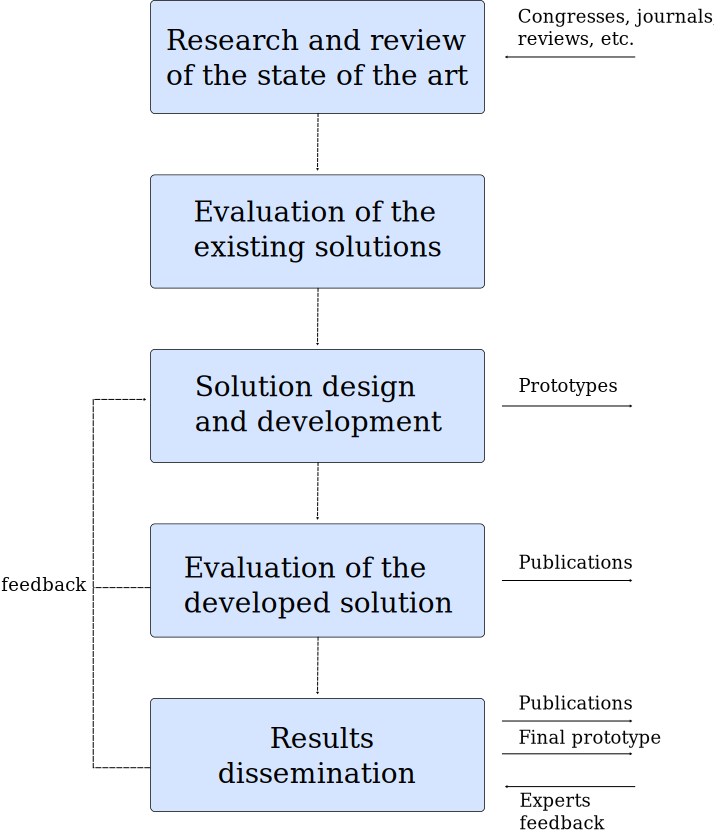
\includegraphics[width=0.60\textwidth]{methodology.pdf}
\caption{Followed research methodology.}
\label{fig:methodology}
\end{figure}
\input{1_introduction/6_outline}